Quando si progetta una applicazione web che offre un servizio, bisogna sempre porre molta attenzione a non introdurre nel sistema i cosiddetti \textit{colli di bottiglia}, cio� componenti dell'architettura che non riescono a sopportare il carico delle richieste in arrivo dagli utenti.

Una tecnica piuttosto efficace per evitare i colli di bottiglia, consiste nel realizzare un \textit{disaccoppiamento} delle varie componenti presenti nel sistema. Una applicazione ben disaccoppiata � una applicazione nella quale ogni singolo componente svolge una funzione specifica e comunica con le altre parti del sistema secondo protocolli predefiniti. Disaccoppiare quindi non � sempre facile, perch� � necessario costruire infrastrutture che permettano alle varie parti, ormai slegate, di comunicare tra loro.

RabbitMQ \cite{website:RabbitMQ} � un software che permette di realizzare, configurare e monitorare complessi sistemi di code di messaggi. Il suo utilizzo permette di realizzare una infrastruttura nella quale le diverse parti di un sistema possano comunicare tra loro scambiandosi messaggi attraverso le code utilizzando un protocollo determinato dallo sviluppatore.\\

\begin{figure}[h]
\centering

\includegraphics[width=0.7\linewidth]{./img/rabbit_header_logo}
\caption[Il logo di RabbitMQ]{Il logo di RabbitMQ}
\label{fig:rabbit-logo}
\end{figure}

L'utilizzo di RabbitMQ fornisce un vantaggio evidente in termini di flessibilit�: � possibile agganciare o rimuovere parti da un sistema attivo senza comprometterne l'intero funzionamento.

La flessibilit� non � l'unico vantaggio, infatti RabbitMQ permette di ottenere architetture perfettamente gestibili su sistemi di tipo \textit{Platform as a Service} (PaaS), sui quali si pu� decidere di aumentare o diminuire dinamicamente le risorse fornite ad un sistema in produzione in accordo con il numero di richieste utente da soddisfare. 

RabbitMQ permette di costruire \textit{pattern} di comunicazione tra processi, i pi� utilizzati sono quelli riportati di seguito.

\subsubsection{Work Queues}

L'idea alla base questo tipo di configurazione, chiamata anche \textit{Task Queues}, consiste nell'evitare picchi nel carico di lavoro e risorse del sistema, dovuti allo svolgimento di una operazione e all'attesa del suo completamento. Per ovviare a questo problema si configura un sistema nel quale esiste un produttore di dati e uno o pi� consumatori.\\

\begin{figure}[h]
\centering
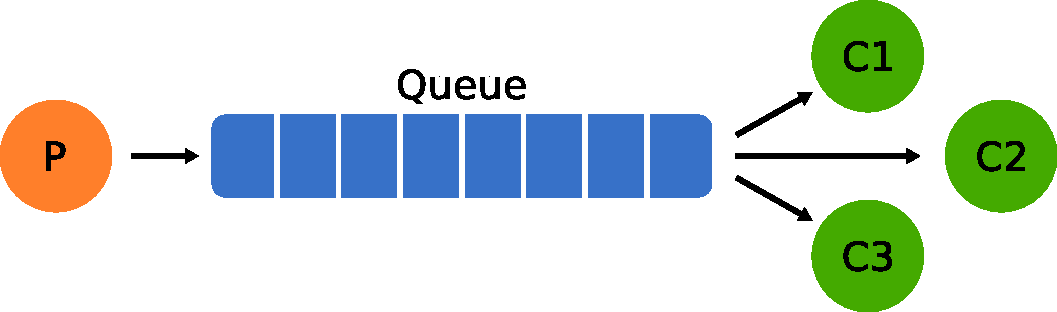
\includegraphics[width=0.7\linewidth]{./img/rabbit-workers}
\caption[Work Queues in RabbitMQ]{Work Queues in RabbitMQ}
\label{fig:rabbit-work-queues}
\end{figure}

In figura \ref{fig:rabbit-work-queues} vediamo una rappresentazione schematica di questo tipo di configurazione. All'arrivo di una richiesta di elaborazione, il produttore (P) invia un messaggio sulla coda. I consumatori (C1, C2 e C3) in attesa estraggono un messaggio dalla coda e lo elaborano.

Nella sua configurazione base, la coda esegue un \textit{load-balancing} dei messaggi, questo significa che fornisce esattamente lo stesso quantitativo di messaggi, e quindi di carico di lavoro, ad ogni consumatore.

RabbitMQ permette di variare il numero di consumatori in ascolto sulla coda dinamicamente, a \textit{runtime}. Non appena un nuovo consumatore si registra per la ricezione dei messaggi, il carico di lavoro viene automaticamente ricalcolato in modo da essere costante per tutti i nodi.

Il load-balancing automatico e la possibilit� di sottoscrivere consumatori a runtime diventano funzionalit� molto importanti in presenza di sistemi attivi su PaaS. All'aumentare delle richieste, infatti, il sistema potrebbe in automatico attivare nuovi consumatori e sottoscriverli, ottenendo in questo modo un sistema altamente scalabile. 

\subsubsection{Publish/Subscribe}

Questa configurazione si ispira al concetto di \textit{abbonamento}, l'idea di base infatti � poter inviare il medesimo messaggio a pi� destinatari.\\

\begin{figure}[h]
\centering
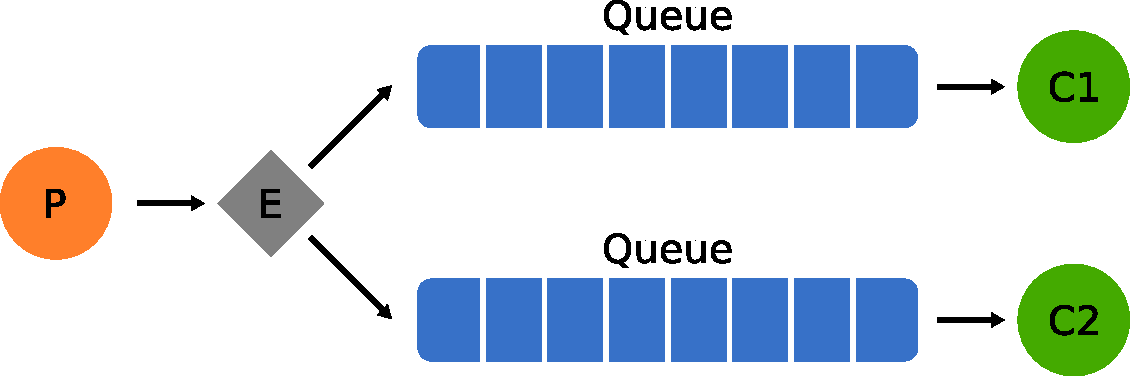
\includegraphics[width=0.7\linewidth]{./img/rabbit-pub-sub}
\caption[Publish/Subscribe in RabbitMQ]{Publish/Subscribe in RabbitMQ}
\label{fig:rabbit-publish-subscribe}
\end{figure}

La figura \ref{fig:rabbit-publish-subscribe} mostra una rappresentazione del sistema Publish/Subscribe. A differenza del modello \textit{Work Queues}, qui � stato aggiunto un nuovo attore: un \textit{exchange} (E) il cui compito � duplicare i messaggi e inviarli a tutte le code ad esso connesse.

In questo caso il produttore di messaggi (P) invia un messaggio ad un exchange (E), il quale lo duplica e lo invia a tutte le code ad esso connesse. I consumatori in ascolto (C1 e C2), riceveranno lo stesso messaggio.\\

%TODO
% il routing dei messaggi? (per� non l'ho usato)

Nella sezione \ref{Architettura_del_sistema} vedremo nel dettaglio la configurazione di RabbitMQ utilizzata per realizzare Mole.io e quali tecniche abbiamo messo in atto per permettere al sistema di essere installato su una piattaforma di tipo PaaS.

